% class
\documentclass[a4paper,12pt,xelatex,ja=standard]{bxjsarticle}

% packages
%% mathematical notations
\usepackage{amsthm,amsmath,amssymb,amsfonts} % mathematical notations
\usepackage{bm} % bold character
\usepackage{latexsym} % more mathematical notations
\usepackage{physics} % physical notations
%% graphs
\usepackage{graphicx, xcolor} % graph
\usepackage{circuitikz} % for circuit elements
\usepackage{float} % positioning of graphs
\usepackage{siunitx} % SI units
\usepackage{tikz} % graphic elements
\usepackage{wrapfig} % must be after float package.
%% type system
\usepackage{bussproofs} % proof tree
%% code
\usepackage[ruled,vlined]{algorithm2e} % pseudo code
\usepackage{listings} % source code
\usepackage{inconsolata}
\lstset{
  basicstyle=\footnotesize,
  numbers=left,
  frame={tb}
}

% Basic information
\title{電子情報学専攻 \, 専門 \\ 平成24年 \, 解答・解説}
\author{diohabara}
\date{\today}

\begin{document}
\maketitle

\section*{第1問\ 電気・電子回路}

\section*{第2問\ 論理回路}
\subsection*{(1)}
順序回路とは過去の入力によって決まる状態と現在の入力によって出力が決まる回路である。

\subsection*{(2)}

JKフリップフロップの特性表は以下の通りである。

\begin{table}[H]
  \begin{tabular}{|l|l|l|}
  \hline
  J & K & Q                  \\ \hline \hline
  0 & 0 & Q (hold)           \\ \hline
  0 & 1 & 0 (reset)          \\ \hline
  1 & 0 & 1 (set)            \\ \hline
  1 & 1 & $\overline{Q}$ (toggle) \\ \hline
  * & * & Q (hold)           \\ \hline
  \end{tabular}
\end{table}

また、8進カウンタの動作は以下の表の通りになる。

\begin{table}[H]
  \centering
  \begin{tabular}{|l|l|l|l|l|l|l|}
  \hline
  $n$ & $Q^n_2$ & $Q^n_1$ & $Q^n_0$ & $Q^n_2 \to Q^{n+1}_2$ & $Q^n_1 \to Q^{n+1}_1$ & $Q^n_0 \to Q^{n+1}_0$ \\ \hline \hline
  0 & 0 & 0 & 0 & $0 \to 0$ (hold)   & $0 \to 0$ (hold)   & $0 \to 1$ (toggle) \\ \hline
  1 & 0 & 0 & 1 & $0 \to 0$ (hold)   & $0 \to 1$ (toggle) & $1 \to 0$ (toggle) \\ \hline
  2 & 0 & 1 & 0 & $0 \to 0$ (hold)   & $1 \to 1$ (hold)   & $0 \to 1$ (toggle) \\ \hline
  3 & 0 & 1 & 1 & $0 \to 1$ (toggle) & $1 \to 0$ (toggle) & $1 \to 0$ (toggle) \\ \hline
  4 & 1 & 0 & 0 & $1 \to 1$ (hold)   & $0 \to 0$ (hold)   & $0 \to 1$ (toggle) \\ \hline
  5 & 1 & 0 & 1 & $1 \to 1$ (hold)   & $0 \to 1$ (toggle) & $1 \to 0$ (toggle) \\ \hline
  6 & 1 & 1 & 0 & $1 \to 1$ (hold)   & $1 \to 1$ (hold)   & $0 \to 1$ (toggle) \\ \hline
  7 & 1 & 1 & 1 & $1 \to 0$ (toggle) & $1 \to 0$ (toggle) & $1 \to 0$ (toggle) \\ \hline
  8 & 0 & 0 & 0 & $0 \to 0$ (hold)   & $0 \to 0$ (hold)   & $0 \to 1$ (toggle) \\ \hline
  \end{tabular}
\end{table}

表のtoggleとなっている際の$Q_0, Q_1, Q_2$に注目して、以下の式が成り立つ。

\begin{equation*}
  \centering
  \begin{split}
    &J_0 = K_0 = 1 \\
    &J_1 = K_1 = Q_0 \\
    &J_2 = K_2 = Q_1 Q_0
  \end{split}
\end{equation*}

以上より求める8進カウンタの回路は以下の通り。

\begin{figure}[H]
  \centering
  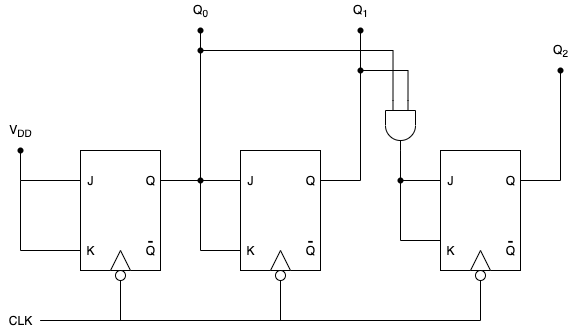
\includegraphics[width=11cm]{images/8_counter.png}
\end{figure}

\subsection*{(3)}

求める同期式5進カウンタの動作表は次の通り。

\begin{table}[H]
  \centering
  \begin{tabular}{|l|l|l|l|l|l|l|}
  \hline
  $n$ & $Q^n_2$ & $Q^n_1$ & $Q^n_0$ & $Q^n_2 \to Q^{n+1}_2$ & $Q^n_1 \to Q^{n+1}_1$ & $Q^n_0 \to Q^{n+1}_0$ \\ \hline \hline
  0 & 0 & 0 & 0 & $0 \to 0$ (hold)   & $0 \to 0$ (hold)   & $0 \to 1$ (toggle) \\ \hline
  1 & 0 & 0 & 1 & $0 \to 0$ (hold)   & $0 \to 1$ (toggle) & $1 \to 0$ (toggle) \\ \hline
  2 & 0 & 1 & 0 & $0 \to 0$ (hold)   & $1 \to 1$ (hold)   & $0 \to 1$ (toggle) \\ \hline
  3 & 0 & 1 & 1 & $0 \to 1$ (toggle) & $1 \to 0$ (toggle) & $1 \to 0$ (toggle) \\ \hline
  4 & 1 & 0 & 0 & $1 \to 0$ (toggle) & $0 \to 0$ (hold)   & $0 \to 0$ (hold)   \\ \hline
  5 & 0 & 0 & 0 & $0 \to 0$ (hold)   & $0 \to 0$ (hold)   & $0 \to 1$ (toggle) \\ \hline
  \end{tabular}
\end{table}

表のtoggleとなっている際の$Q_0, Q_1, Q_2$に注目して、以下の式が成り立つ。

\begin{equation*}
  \begin{split}
    &J_0 = K_0 = \overline{Q_2} \\
    &J_1 = K_1 = Q_0 \\
    &J_2 = Q_1 Q_0 \\
    &K_2 = \overline{Q_2}
  \end{split}
\end{equation*}

以上より求める5進カウンタの回路は以下の通り。

\begin{figure}[H]
  \centering
  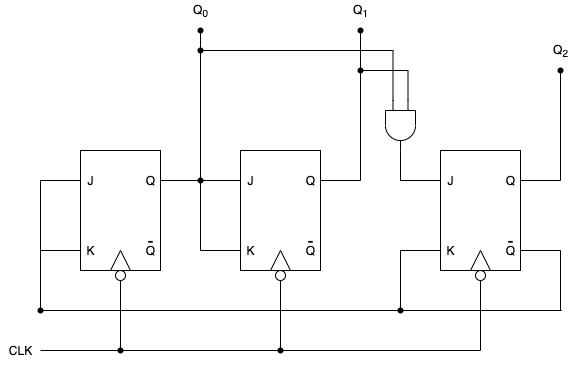
\includegraphics[width=11cm]{images/5_counter.png}
\end{figure}

\subsection*{(4)}
本題の回路の動作表は以下の通り。
\begin{table}[H]
  \begin{tabular}{|l|l|l|l|l|l|l|}
  \hline
  $n$ & $Q^n_2$ & $Q^n_1$ & $Q^n_0$ & $Q^n_2 \to Q^{n+1}_2$ & $Q^n_1 \to Q^{n+1}_1$ & $Q^n_0 \to Q^{n+1}_0$ \\ \hline \hline
  0 & 1 & 1 & 0 & $1 \to 0$ (toggle) & $1 \to 0$ (toggle) & $0 \to 1$ (toggle) \\ \hline
  1 & 0 & 0 & 1 & $0 \to 0$ (hold)   & $0 \to 0$ (hold)   & $1 \to 0$ (toggle) \\ \hline
  2 & 0 & 0 & 0 & $0 \to 0$ (hold)   & $0 \to 1$ (toggle) & $0 \to 0$ (hold)   \\ \hline
  3 & 0 & 1 & 0 & $0 \to 1$ (toggle) & $1 \to 0$ (toggle) & $0 \to 1$ (toggle) \\ \hline
  4 & 1 & 0 & 1 & $1 \to 1$ (hold)   & $0 \to 1$ (toggle) & $1 \to 0$ (toggle) \\ \hline
  5 & 1 & 1 & 0 & $1 \to 0$ (toggle) & $1 \to 0$ (toggle) & $0 \to 1$ (toggle) \\ \hline
  \end{tabular}
\end{table}

表のtoggleとなっている際の$Q_0, Q_1, Q_2$に注目して、以下の式が成り立つ。

\begin{equation*}
  \begin{split}
    &J_0 = K_0 = Q_0 \overline{Q_1} + \overline{Q_0} Q_1 \\
    &J_1 = K_1 = \overline{Q_0} + \overline{Q_1} Q_2 \\
    &J_2 = Q_1 \\
    &K_2 = \overline{Q_0} \\
  \end{split}
\end{equation*}

以上より求める本題の回路は次の通り。

\begin{figure}[H]
  \centering
  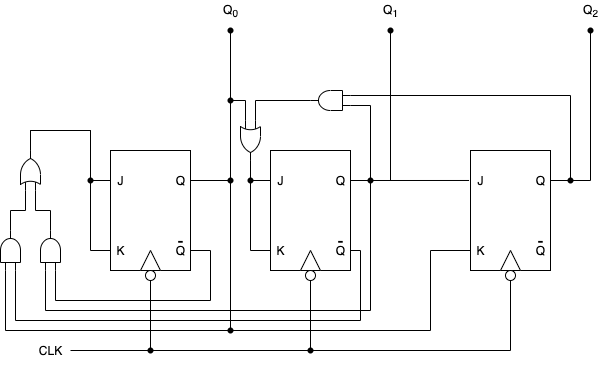
\includegraphics[width=11cm]{images/2013_counter.png}
\end{figure}

\section*{第3問\ アルゴリズム}
\subsection*{(1)}
  \subsubsection*{隣接行列による表現}
  隣接行列とは行列の$i$行$j$列の成分が$1$であるとき頂点$i$から頂点$j$へ辺があり、$0$であるときはないことを表現している。
  \[
    \begin{bmatrix}
    % 0   1   2   3   4   5
      0 & 1 & 0 & 1 & 1 & 0 \\
      0 & 0 & 1 & 1 & 0 & 1 \\
      1 & 0 & 0 & 0 & 1 & 0 \\
      0 & 0 & 1 & 0 & 0 & 1 \\
      1 & 0 & 0 & 0 & 0 & 0 \\
      0 & 0 & 1 & 0 & 1 & 0 \\
    \end{bmatrix}
  \]

  \subsubsection*{隣接リストによる表現}
  隣接リストは各頂点から出ている辺の行き先をリストにして表現したもの。
  \begin{figure}[H]
    \centering
    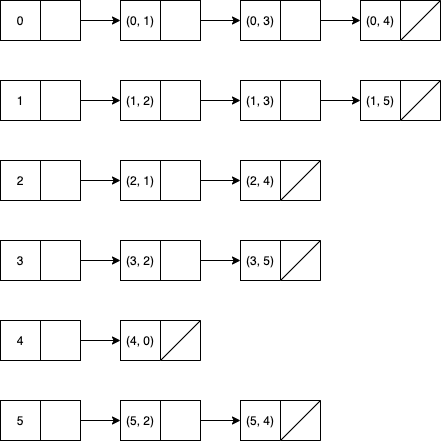
\includegraphics[width=9cm]{images/adjacency_list.png}
  \end{figure}

\subsection*{(2)}
頂点の数を$|V|$とし辺の数を$|E|$とする。隣接行列、隣接リストで必要なメモリはそれぞれ$|V| \times |V|$、$|V| + |E|$である。\\
この問題の場合、$|V| \times |V| = 6^2 = 36, |E| = 6 + 13 = 19$であるから、図1の有向グラフについてよりメモリ容量が必要な表現は隣接行列。

\subsection*{(3)}
(2)で説明したように、頂点数が$N$のとき辺の数を$x$として、隣接行列と隣接リストのメモリ容量が同じになるならば$N + x = N^2$が成り立つ。
よって、$x = N(N - 1)$。\\
また問題の条件から自己ループも多重辺もないので、ある頂点から伸びる辺は最大で$N-1$。頂点数は$N$であるからこの有向グラフの各頂点はそれ以外の全ての頂点と繋がっている。したがって、必ず弱連結となる。

\subsection*{(4)}
擬似コードに従って深さ優先探索をすると以下のような探索木が図示できる。\\
ただし、探索した順番は上から下、左から右であり、丸ノードは探索に成功したノードで四角ノードは探索に失敗したノードである。
\begin{center}
  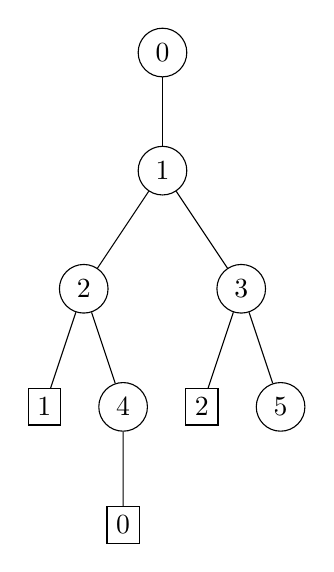
\begin{tikzpicture}[
    level 1/.style={sibling distance=30mm},
    level 2/.style={sibling distance=20mm},
    level 3/.style={sibling distance=10mm},
    node_ok/.style={circle,draw},
    node_no/.style={rectangle,draw}
  ]
    \node[node_ok] {0}
      child { node[node_ok] {1}
        child { node[node_ok] {2}
          child { node[node_no] {1} }
          child { node[node_ok] {4}
            child { node[node_no] {0} }
          }
        }
        child { node[node_ok] {3}
          child { node[node_no] {2} }
          child { node[node_ok] {5} }
        }
      }
    ;
  \end{tikzpicture}
\end{center}

\subsection*{(5)}
以下のように有向サイクルを検出するアルゴリズムは書ける。
\begin{lstlisting}[language=Python, caption="有向サイクル検出アルゴリズム"]
def find_cycle(vertices: list[Vertex], edges: list[Edge]) -> list[Vertex]:
    for v in vertices:
        for from_v, to_v in edges[v]:
            cycle_vs = dfs(from_v, from_v, edges)
            if cycle_vs:
                return cycle_vs
    return []

def dfs(initial_v: Vertex, current: Vertex, edges: list[Edge]) -> list[Vertex]:
    for from_v, to_v in edges[current]:
        cycle_vs = dfs(initial_v, to_v, edges)
        if initial_v == to_v:
            return cycle_vs
    return []
\end{lstlisting}

\section*{第4問\ ネットワーク}

\section*{第5問\ 情報理論}
\subsection*{(1)}
状態遷移図は以下の通り。
\begin{center}
  \usetikzlibrary {automata,positioning}
  \begin{tikzpicture}[
      ->,
      >={Stealth[round]},
      auto,
      every state/.style={draw}
    ]
    \node[state] (R) {R};
    \node[state] (G) [below right=of R] {G};
    \node[state] (B) [below left=of R] {B};

    \path
      (R)
        edge node {0.2} (G)
        edge [loop above] node {0.8} (R)
      (G)
        edge [loop right] node {0.9} (G)
        edge node {0.1} (B)
      (B)
        edge [loop left] node {0.9} (B)
        edge node {0.1} (R)
    ;

    \node [right=1cm,text width=7cm] at (G)
    {
      \begin{itemize}
        \item Rの直後には、RとGのどちらかが、それぞれ0.8と0.2の確率で光る。
        \item Gの直後には、GとBのどちらかが、それぞれ0.9と0.1の確率で光る。
        \item Bの直後には、BとRのどちらかが、それぞれ0.9と0.1の確率で光る。
      \end{itemize}
    };
  \end{tikzpicture}
\end{center}

\subsection*{(2)}
求める定常状態確率をそれぞれ$\overline{P_R}$、$\overline{P_G}$
、$\overline{P_B}$とする。\\
状態遷移図から定常状態確率は次のような方程式が立てられる。

\begin{equation*}
  \begin{split}
    \overline{P_R} &= 0.8 \overline{P_R} + 0.1 \overline{P_B} \\
    \overline{P_G} &= 0.9 \overline{P_G} + 0.2 \overline{P_R} \\
    \overline{P_B} &= 0.9 \overline{P_R} + 0.2 \overline{P_G}
  \end{split}
\end{equation*}

変形して

\begin{equation*}
  \begin{split}
    2\overline{P_R} &= \overline{P_B} \\
    \overline{P_G} &= 2 \overline{P_R} \\
    \overline{P_B} &= \overline{P_G}
  \end{split}
\end{equation*}

とすると、$\overline{P_R} : \overline{P_G} : \overline{P_B} = 1 : 2 : 2$となる。
したがって、$\overline{P_R} + \overline{P_G} + \overline{P_B} = 1$であるから
\begin{equation*}
  \begin{split}
    \overline{P_R} &= 0.2 \\
    \overline{P_G} &= 0.4 \\
    \overline{P_B} &= 0.4 \\
  \end{split}
\end{equation*}

\subsection*{(3)}

状態遷移図より考えられる点灯を2つずつまとめた系列は$RR$、$RG$、$GG$、$GB$、$BB$、$BR$の6通りである。
それぞれの系列の確率を$P_{RR}$、$P_{RG}$、$P_{GG}$、$P_{GB}$、$P_{BB}$、$P_{BR}$とおきこれらを最も効率が良くなるように符号を設計する。\\

(2)より定常状態確率は求まっており、2つずつまとめた系列は1つ目の点灯から2つ目の点灯へ遷移する条件付き確率であるからそれぞれの確率は次の通り。

\begin{equation*}
  \begin{split}
    P_{RR} &= 0.8 \overline{P_R} = 0.16 \\
    P_{RG} &= 0.2 \overline{P_R} = 0.04 \\
    P_{GG} &= 0.9 \overline{P_G} = 0.36 \\
    P_{GB} &= 0.1 \overline{P_G} = 0.04 \\
    P_{BB} &= 0.9 \overline{P_B} = 0.36 \\
    P_{BR} &= 0.1 \overline{P_B} = 0.04 \\
  \end{split}
\end{equation*}

以上より、確率が高いノードから低いノードに並べて、ノードのうち確率が最も低いノードを順番に合併させれば次のようにハフマン符号を設計できる。\\
このとき、右端のノードから辿って左端のノードに行くとき上の辺を通るとき符号0、下の辺を通るとき符号1を付ければ2元符号は最も効率よく設計できる。\\

\begin{figure}[H]
  \centering
  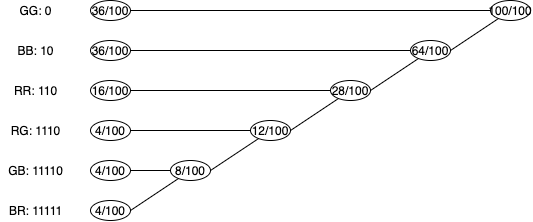
\includegraphics[width=11cm]{images/huffman_tree2013.png}
\end{figure}

2点灯系列あたりの平均符号長は
\[
  3P_{RR} + 4P_{RG} + 1P_{GG} + 5P_{GB} + 2P_{BB} + 5P_{BR} = 2.12
\]
よって、1点灯系列あたりの平均符号長は$1.06$[bit]

\subsection*{(4)}
% (3)と同様に系列ごとの確率を定め、定常状態確率から
% \begin{equation*}
%   \begin{split}
%     P_{RG} &= 0.2 \overline{P_R} =  \\
%     P_{RRG} &= 0.2 \cdot 0.8 \overline{P_R} = 0.04 \\
%     P_{RRR} &= 0.8 \cdot 0.8 \overline{P_R} = 0.36 \\
%     P_{GB} &= 0.1 \overline{P_G} = 0.04 \\
%     P_{GGB} &= 0.1 \cdot 0.9 \overline{P_G} = 0.36 \\
%     P_{GGG} &= 0.9 \cdot 0.9 \overline{P_G} = 0.04 \\
%     P_{BR} &= 0.1 \overline{P_B} = 0.04 \\
%     P_{BBR} &= 0.1 \cdot 0.9 \overline{P_B} = 0.36 \\
%     P_{BBB} &= 0.9 \cdot 0.9 \overline{P_B} = 0.04 \\
%   \end{split}
% \end{equation*}
TODO

\subsection*{(5)}
各々の色とその次の点灯についてのエントロピーは以下の通りになる。

Rから始まるときのエントロピーは
\begin{equation*}
  \begin{split}
    H_{R}
      &= -(0.8 \log{\frac{8}{10}} + 0.2 \log{\frac{2}{10}}) \\
      &= -(0.8 (\log 8 - \log10) + 0.2 (\log 2 - \log10)) \\
      &= -(0.8 (3 - \log10) + 0.2 (1 - \log10)) \\
      &= -(2.6 - \log10)
  \end{split}
\end{equation*}

Gから始まるときのエントロピーは
\begin{equation*}
  \begin{split}
    H_{G}
      &= -(0.9 \log{\frac{9}{10}} + 0.1 \log{\frac{1}{10}}) \\
      &= -(0.9 (\log 9 - \log 10) + 0.1 (\log 1 - \log 10)) \\
      &= -(0.9 (2 \log 3 - \log 10) + 0.1 (0 - \log 10)) \\
      &= -(1.8 \log 3 - \log 10) \\
  \end{split}
\end{equation*}

Bから始まるときのエントロピーは
\begin{equation*}
  \begin{split}
    H_{B}
      &= -(0.9 \log{\frac{9}{10}} + 0.1 \log{\frac{1}{10}}) \\
      &= -(0.9 (\log 9 - \log 10) + 0.1 (\log 1 - \log 10)) \\
      &= -(0.9 (2 \log 3 - \log 10) + 0.1 (0 - \log 10)) \\
      &= -(1.8 \log 3 - \log 10) \\
  \end{split}
\end{equation*}

定常状態確率は(2)で求めた通り。以上から求めるエントロピー$H$は

\begin{equation*}
  \begin{split}
    H &= 0.2 H_R + 0.4 H_G + 0.4 H_B \\
      &= -(0.2 (2.6 - \log 10) + 0.8 (1.8 \log 3 - \log 10) \\
      &= -(0.52 + 1.44 \log 3 - \log 10 ) \\
      &= -(0.52 + 1.44 \log 3 - \log 2 - \log 5 ) \\
      &= -(0.52 + 1.44 \cdot 1.58 - 1 - 2.32 ) \\
      &= 0.5248
  \end{split}
\end{equation*}

\end{document}

